\documentclass[11pt]{article}
\usepackage{amsmath,tikz}
\usetikzlibrary{arrows.meta,positioning}
\begin{document}
\section*{Residual Curve Dependency Map (Directive 011)}
\begin{center}
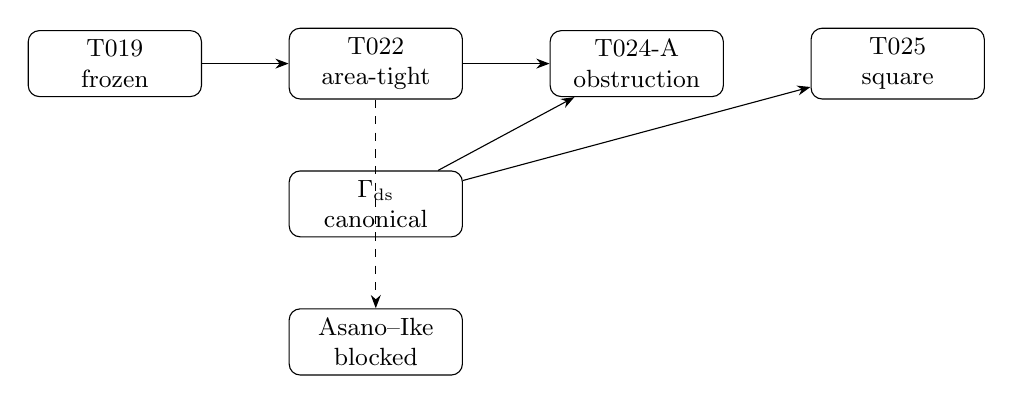
\begin{tikzpicture}[
  node distance=0.9cm and 1.1cm,
  box/.style={draw,rounded corners,align=center,minimum width=2.2cm,font=\small}
]
  \node[box] (t019) {T019\\frozen};
  \node[box, right=of t019] (t022) {T022\\area-tight};
  \node[box, right=of t022] (t024) {T024-A\\obstruction};
  \node[box, below=of t022] (ds) {$\Gamma_{\mathrm{ds}}$\\canonical};
  \node[box, right=of t024] (t025) {T025\\square};
  \node[box, below=of ds] (ai) {Asano--Ike\\blocked};
  \draw[-{Stealth}] (t019) -- (t022);
  \draw[-{Stealth}] (t022) -- (t024);
  \draw[-{Stealth}] (ds) -- (t024);
  \draw[-{Stealth}] (ds) -- (t025);
  \draw[-{Stealth},dashed] (t022) -- (ai);
\end{tikzpicture}
\end{center}
\end{document}
